% !TEX encoding = UTF-8 Unicode
%%%%%%%%%%%%%%%%%%%%%%%%%%%%%%%%%%%%%%%%%
% Beamer Presentation
% LaTeX Template
% Version 1.0 (10/11/12)
%
% This template has been downloaded from:
% http://www.LaTeXTemplates.com
%
% License:
% CC BY-NC-SA 3.0 (http://creativecommons.org/licenses/by-nc-sa/3.0/)
%
%%%%%%%%%%%%%%%%%%%%%%%%%%%%%%%%%%%%%%%%%

%----------------------------------------------------------------------------------------
%	PACKAGES AND THEMES
%----------------------------------------------------------------------------------------

\documentclass{beamer}

\mode<presentation> {

% The Beamer class comes with a number of default slide themes
% which change the colors and layouts of slides. Below this is a list
% of all the themes, uncomment each in turn to see what they look like.

%\usetheme{default}
%\usetheme{AnnArbor}
%\usetheme{Antibes}
%\usetheme{Bergen}
%\usetheme{Berkeley}
%\usetheme{Berlin}
%\usetheme{Boadilla}
%\usetheme{CambridgeUS}
%\usetheme{Copenhagen}
%\usetheme{Darmstadt}
%\usetheme{Dresden}
%\usetheme{Frankfurt}
%\usetheme{Goettingen}
%\usetheme{Hannover}
%\usetheme{Ilmenau}
%\usetheme{JuanLesPins}
%\usetheme{Luebeck}
\usetheme{Madrid}
%\usetheme{Malmoe}
%\usetheme{Marburg}
%\usetheme{Montpellier}
%\usetheme{PaloAlto}
%\usetheme{Pittsburgh}
%\usetheme{Rochester}
%\usetheme{Singapore}
%\usetheme{Szeged}
%\usetheme{Warsaw}

% As well as themes, the Beamer class has a number of color themes
% for any slide theme. Uncomment each of these in turn to see how it
% changes the colors of your current slide theme.

%\usecolortheme{albatross}
%\usecolortheme{beaver}
%\usecolortheme{beetle}
%\usecolortheme{crane}
%\usecolortheme{dolphin}
%\usecolortheme{dove}
%\usecolortheme{fly}
%\usecolortheme{lily}
%\usecolortheme{orchid}
%\usecolortheme{rose}
%\usecolortheme{seagull}
%\usecolortheme{seahorse}
%\usecolortheme{whale}
%\usecolortheme{wolverine}

%\setbeamertemplate{footline} % To remove the footer line in all slides uncomment this line
%\setbeamertemplate{footline}[page number] % To replace the footer line in all slides with a simple slide count uncomment this line

%\setbeamertemplate{navigation symbols}{} % To remove the navigation symbols from the bottom of all slides uncomment this line
}

\usepackage{graphicx} % Allows including images
\usepackage{booktabs} % Allows the use of \toprule, \midrule and \bottomrule in tables
\usepackage{xeCJK}
\usepackage{color}
\usepackage{listings}
\usepackage{tikz}


%----------------------------------------------------------------------------------------
%	TITLE PAGE
%----------------------------------------------------------------------------------------

\title[数据管理]{数据管理} % The short title appears at the bottom of every slide, the full title is only on the title page

\author{张海宁} % Your name
\institute[计算机科学与技术学院] % Your institution as it will appear on the bottom of every slide, may be shorthand to save space
{
贵州大学 \\ % Your institution for the title page
\medskip
\textit{hnzhang1@gzu.edu.cn} % Your email address
}
\date{\today} % Date, can be changed to a custom date

\begin{document}

\begin{frame}
\titlepage % Print the title page as the first slide
\end{frame}

\begin{frame}
\frametitle{Overview} % Table of contents slide, comment this block out to remove it
\tableofcontents % Throughout your presentation, if you choose to use \section{} and \subsection{} commands, these will automatically be printed on this slide as an overview of your presentation
\end{frame}

%----------------------------------------------------------------------------------------
%	PRESENTATION SLIDES
%----------------------------------------------------------------------------------------
\section{内存管理}
\begin{frame}
\Huge{\centerline{内存管理}}
\end{frame}
\begin{frame}{内存管理概述}
在所有的计算机系统中,\textcolor{red}{内存}都是一种\textcolor{red}{稀缺资源}。而且无论有多少内存,似乎总是不够用,
这就对内存的管理提出了挑战。

联想一下电脑和手机的内存增长史,应用程序所需要占用的内存也在随着内存容量的增长而增加。
%\begin{tikzpicture}
%[mynode/.style={rectangle,draw=blue!50,thick,minimum width=12mm,minimum height=7mm},
%mytext/.style={red,below}]
%\node (a) at (0,0) [mynode] {512M};
%\node (b) at (1.5,0) [mynode] {1G};
%\node (c) at (3,0) [mynode] {2G};
%\node (d) at (4.5,0) [mynode] {4G};
%\node (e) at (6,0) [mynode] {8G};
%\node (f) at (7.5,0) [mynode] {16G};
%\node (h) at (9,0) [mynode] {more};
%\node [mytext] (n1) at (a.south) {2008};
%\node [mytext] (n2) at (b.south) {2009};
%\node [mytext] (n3) at (c.south) {2010};
%\node [mytext] (n4) at (d.south) {2012};
%\node [mytext] (n5) at (e.south) {2015};
%\node [mytext] (n6) at (f.south) {2018};

%\end{tikzpicture}
\end{frame}
\begin{frame}[fragile]{内存分配I}
\begin{block}{使用c语言标准库中的malloc来分配内存}
\begin{lstlisting}
\end{lstlisting}
\#include<stdlib.h>

void *malloc(size\_t size);
\end{block}
\end{frame}
\begin{frame}[fragile]{内存分配II}
\begin{block}{使用c语言标准库中的malloc来分配内存}
\begin{lstlisting}
\end{lstlisting}
\#include<stdlib.h>

void *malloc(size\_t size);
\end{block}
\end{frame}
%------------------------------------------------
\section{文件锁定}
\begin{frame}
\Huge{\centerline{文件锁定}}
\end{frame}
\begin{frame}{文件锁定}
文件锁定是多用户多任务操作系统中一个非常重要的组成部分。如果两个程序同时访问一个文件,一个读一个写,或者都在写,那么非常有可能出现文件内容不一致。
Linux使用文件锁定来解决这个问题。实现文件锁定有两种形式:
\begin{enumerate}
\item
创建锁文件
\item
锁定区域
\end{enumerate}
\end{frame}
\begin{frame}[fragile]{创建锁文件I}
许多应用程序只要能够针对某个资源创建一个锁文件即可,然后其他的程序就可以通过检查这个文件的状态来判断它们自己是否被允许访问这个资源。

为了创建一个用途锁指示器的文件,使用fcntl.h头文件中定义的带O\_CREAT和O\_EXECL标志的open系统调用。这样能保证以一个原子操作同时完成两项工作:确定文件不存在,然后创建它。
\begin{block}{}
\emph{O\_EXCL          error if O\_CREAT and the file exists}
\end{block}
\end{frame}
\begin{frame}[fragile]{创建锁文件II}
\label{lock}
\begin{block}{创建锁文件部分代码}
\begin{lstlisting}
int main(){
 int file_desc, save_errno;	
  file_desc=open("LCK.test",O_RDWR|O_CREAT|O_EXCL,
     S_IRUSR);
  if(file_desc==-1){
   save_errno=errno;
   printf("Open failed with error code %d.\n",
     save_errno);
  }else{
   printf("Open succeeded.\n");
  }
 exit(EXIT_SUCCESS);
}
\end{lstlisting}
\end{block}
\end{frame}
\begin{frame}[fragile]{创建锁文件III}
\begin{block}{执行第\ref{lock}页代码}
\begin{lstlisting}
$ ./lock1 
Open succeeded.
$ ./lock1 
Open failed with error code 17.
\end{lstlisting}
\end{block}
可以看到,第一次运行程序,会成功打开文件,第二次运行就会打开失败,其实不管再运行几次,都会失败。Why?

关于errno的更多信息可以查看第\ref{ferr}页。
\end{frame}
\begin{frame}[fragile]{创建锁文件IV}
\textbf{临界区:}
如果某个程序在执行的时候需要独占某个资源进行某操作,这部分操作被称为临界区,程序在进入临界区之前需要创建锁文件,
在退出临界区之前需要删除(unlink)锁文件。
\begin{block}{临界区代码}
\begin{lstlisting}
void writeAfile(){
 FILE *out = fopen("lcktest2","a");
 char st='a', end='z', c;
 for(c=st;c<end;c++){
  fputc(c,out);  fflush(out);
 }
 fputc('\n',out); fclose(out);
 printf("write done.\n");
}
\end{lstlisting}
\end{block}
\end{frame}
\begin{frame}[fragile]{创建锁文件V}
\begin{block}{普通模式访问代码}
\begin{lstlisting}
int main(){
 int file_desc, tries=2;
 while(tries--){
  writeAfile();
 }
 exit(EXIT_SUCCESS);
}
\end{lstlisting}
\end{block}
\end{frame}
\begin{frame}[fragile]{创建锁文件VI}
\begin{block}{使用锁文件方式}
\begin{lstlisting}
int main(){
 int file_desc, tries=2;
 while(tries--){
  file_desc=open(lock_file,O_RDWR|O_CREAT|O_EXCL,
    S_IRUSR);
  if(file_desc==-1){
   printf("%d : Lock already present.\n",getpid());
   sleep(3);  tries++;
  }else{
   printf("%d : Got access.\n",getpid());
   writeAfile(); close(file_desc);
   unlink(lock_file); sleep(1);
  } } exit(EXIT_SUCCESS);}
\end{lstlisting}
\end{block}
\end{frame}
\begin{frame}[fragile]{创建锁文件VII}
\label{filelock}
\begin{block}{查看结果}
\begin{lstlisting}
普通方式执行程序
$./lock2n & ./lock2n
aabbccddeeffgghhiijjkkllmmnnooppqqrrssttuuvvwwxxyy

abcdeafbcdhefgiijklmnopqjrksltmnopqrstuvwxy
uvwxy
创建锁文件方式执行程序
$./lock2 & ./lock2
abcdefghijklmnopqrstuvwxy
abcdefghijklmnopqrstuvwxy
abcdefghijklmnopqrstuvwxy
abcdefghijklmnopqrstuvwxy
\end{lstlisting}
\end{block}
\end{frame}
\begin{frame}[fragile]{创建锁文件VIII}
通过第\ref{filelock}页,可以看出,通过创建锁文件的方式,达到了一个程序单独占用某个文件的目的,确保了同一时间段只能有一个程序来独占一个文件进行操作。
\end{frame}
\begin{frame}{锁定区域}
创建锁文件的方式会造成对文件的\textcolor{red}{独占式访问},这不适合用来访问大型共享文件。比如一个日志文件,随时都可能会有数据写入,为了让其他程序也能读取这个不会停止写入的文件,需要有一种协调机制来提供对一个文件的\textcolor{red}{同时访问}。

文件中的\textcolor{red}{锁定区域}可以用来解决这个问题,即文件的一部分被锁定,但其他程序可以访问这个文件的其他部分。这种机制被称为\textcolor{red}{文件段锁定或文件区锁定}。

\begin{block}{两个系统调用}
\begin{enumerate}
\item
lockf
\item
fcntl

最常用
\end{enumerate}
\end{block}
\end{frame}
\begin{frame}[fragile]{fcntl}
\begin{block}{原型}
\begin{lstlisting}
#include<fcntl.h>

int fcntl(int fildes, int cmd, ...);
\end{lstlisting}
\end{block}
fcntl对一个打开的文件描述符进行操作,并根据cmd参数的设置完成不同的任务。其有三个用于文件锁的命令:
\begin{enumerate}
\label{flckcmd}
\item
F\_GETLK  获取锁信息。若失败,返回-1。
\item
F\_SETLK 设置锁。若失败,返回-1。
\item
F\_SETLKW 设置锁,直到成功。
\end{enumerate}
\end{frame}
\begin{frame}{flock}
当使用第\ref{flckcmd}页这些参数的时候,第三个参数必须是一个指向flock结构的指针,fcntl完整的原型应该是:

\fbox{int fcntl(int fildes, int cmd, struct flock *flk)}

flock(file lock)结构依赖于具体的实现,但至少包含以下成员:
\begin{enumerate}
\item
short l\_type;
\begin{itemize}
\item
F\_RDLCK  共享(读)锁。
\item
F\_UNLCK 解锁。
\item
F\_WRLCK 独占(写)锁。
\end{itemize}
\item
short l\_whence  SEEK\_SET SEEK\_CUR SEEK\_END。
\item
off\_t l\_start 相对于whence的偏移量(字节)。
\item
off\_t l\_len 字节个数。
\item
pid\_t l\_pid 记录持有锁的进程号。
\end{enumerate}
\end{frame}
\begin{frame}{锁定状态下的读写操作}
当对文件的区域加锁之后,访问文件应当使用read和write调用,不要使用fread和fwrite,因为后者会缓存比要求更多的数据。

\end{frame}
\begin{frame}{使用fcntl锁定文件I}
\begin{tikzpicture}
\node (a) at (0,0) {0} ;
\node (b) at (1,0) {10};
\node (c) at (3,0) {30};
\node (d) at (4,0) {40};
\node (e) at (5,0) {50};
\node (f) at (10,0) {100};
\node (g) at (10,5) {};
\node (h) at (5,5) {};
\node (i) at (4,5) {};
\node (j) at (3,5) {};
\node (k) at (1,5) {};
\node (l) at (0,5) {};
\draw (a) -- (b) --(c) -- (d) --(e) -- (f) --(g) -- (h) --(i) -- (j) --(k) -- (l) --(a);
\draw [red] (b) -- (k);
\draw [red] (c) -- (j);
\draw [red] (d) -- (i);
\draw [red] (e) -- (h);
\node (rdlck) at (2,2){F\_RDLCK}; 
\node (wrlck) at (4.5,2) [rotate=45]{F\_WRLCK};
\end{tikzpicture}
\end{frame}
\begin{frame}[fragile]{使用fcntl锁定文件II}
\begin{block}{头文件及声明}
\begin{lstlisting}
//lock3.c
#include<unistd.h>
#include<fcntl.h>
#include<stdlib.h>
#include<stdio.h>
const char *test_file="lck3.lock";
int main(){
 int file_desc;
 int byte_count;
 char * byte_to_write="A";
 struct flock region_1;
 struct flock region_2;
 int res;
\end{lstlisting}
\end{block}
\end{frame}
\begin{frame}[fragile]{使用fcntl锁定文件III}
\begin{block}{打开一个文件}
\begin{lstlisting}
//open a file discription
 file_desc=open(test_file, O_RDWR | O_CREAT, 0666);
 if(!file_desc){
  fprintf(stderr,"Unable to open %s.\n",test_file);
  exit(EXIT_FAILURE);
 }
// write some data
 for(byte_count=0;byte_count<100;byte_count++){
  write(file_desc, byte_to_write, 1);
 }
\end{lstlisting}
\end{block}
\end{frame}
\begin{frame}[fragile]{使用fcntl锁定文件IV}
\begin{block}{设置锁信息}
\begin{lstlisting}
//set region 1 as read lock
 region_1.l_type = F_RDLCK;
 region_1.l_whence = SEEK_SET;
 region_1.l_start = 10;
 region_1.l_len=20;

//set region 2 as write lock	
 region_2.l_type = F_WRLCK;
 region_2.l_whence = SEEK_SET;
 region_2.l_start = 40;
 region_2.l_len=10;
\end{lstlisting}
\end{block}
\end{frame}
\begin{frame}[fragile]{使用fcntl锁定文件V}
\begin{block}{锁定文件}
\begin{lstlisting}
//lock file
 printf("Process %d locking file.\n",getpid());
 res = fcntl(file_desc, F_SETLK, &region_1);
 if(res==-1){
  fprintf(stderr,"proc %d failed to lock region 1.\n"
    , getpid());
 }
 res = fcntl(file_desc, F_SETLK, &region_2);
 if(res==-1){
  fprintf(stderr,"proc %d failed to lock region 2.\n"
    , getpid());
 }


\end{lstlisting}
\end{block}
\end{frame}
\begin{frame}[fragile]{使用fcntl锁定文件VI}
\begin{block}{关闭文件}
\begin{lstlisting}
//sleep
 sleep(20);
 printf("process %d prepare to close the file.\n"
   , getpid());
 close(file_desc);
 exit(EXIT_SUCCESS);
}
\end{lstlisting}
\end{block}
\underline{程序对某个文件拥有的所有锁都将在相应的文件描述符关闭时自动清除。}
\end{frame}
\begin{frame}{测试文件上的锁}
编写一个lock4.c文件,在lock3.c的程序在文件lck3.lock上设置锁的同时,使用lock4.c的程序再加锁,对比结果。
\end{frame}
\begin{frame}[fragile]{测试文件上的锁I}
\begin{block}{头文件及声明}
\begin{lstlisting}
//lock4.c
#include<unistd.h>
#include<fcntl.h>
#include<stdlib.h>
#include<stdio.h>
const char *test_file="lck3.lock";
#define SIZE_TO_TRY 5
void show_lock_info(struct flock *to_show);
int main(){
 int file_desc;
 struct flock region_to_test;
 int res;
 int start_byte;
\end{lstlisting}
\end{block}
\end{frame}
\begin{frame}[fragile]{测试文件上的锁II}
\begin{block}{打开一个文件,并开始一个循环}
\begin{lstlisting}
//open a file discription
 file_desc=open(test_file, O_RDWR | O_CREAT, 0666);
 if(!file_desc){
  fprintf(stderr,"Unable to open %s.\n",test_file);
  exit(EXIT_FAILURE);
 }
 for(start_byte=0;start_byte<99;
   start_byte+=SIZE_TO_TRY){
\end{lstlisting}
\end{block}
\end{frame}
\begin{frame}[fragile]{测试文件上的锁III}
\begin{block}{设置写锁}
\begin{lstlisting}
//set a write lock	
 region_to_test.l_type = F_WRLCK;
 region_to_test.l_whence = SEEK_SET;
 region_to_test.l_start = start_byte;
 region_to_test.l_len=SIZE_TO_TRY;
 region_to_test.l_pid=-1;	
 \end{lstlisting}
\end{block}
\end{frame}
 \begin{frame}[fragile]{测试文件上的锁IV}
\begin{block}{测试写锁}
\begin{lstlisting}
//test the write lock can be set or not
 printf("Testing the F_WRLCK on region from %d to %d
  \n",start_byte,start_byte+SIZE_TO_TRY);	
 res=fcntl(file_desc,F_GETLK,&region_to_test);
 if(res==-1){
  fprintf(stderr,"F_GETLK(F_WRLCK) failed!\n");
  exit(EXIT_FAILURE);
 }
 if(region_to_test.l_pid!=-1){
  printf("F_WRLCK would fail.F_GETLK returned:\n");
  show_lock_info(&region_to_test);
 }else{
  printf("F_WRLCK - lock would succeed.\n");
 }
\end{lstlisting}
\end{block}
\end{frame}
\begin{frame}[fragile]{测试文件上的锁V}
\begin{block}{设置读锁}
\begin{lstlisting}
//set a read lock
 region_to_test.l_type = F_RDLCK;
 region_to_test.l_whence = SEEK_SET;
 region_to_test.l_start = start_byte;
 region_to_test.l_len=SIZE_TO_TRY;
 region_to_test.l_pid=-1;
\end{lstlisting}
\end{block}
\end{frame}
\begin{frame}[fragile]{测试文件上的锁VI}
\begin{block}{测试读锁}
\begin{lstlisting}
//test the read lock can be set or not
 printf("Testing the F_RDLCK on region from %d to %d
  \n",start_byte,start_byte+SIZE_TO_TRY);	
 res=fcntl(file_desc,F_GETLK,&region_to_test);
 if(res==-1){
  fprintf(stderr,"F_GETLK(F_RDLCK) failed!\n");
  exit(EXIT_FAILURE);
 }
 if(region_to_test.l_pid!=-1){
  printf("F_RDLCK would fail.F_GETLK returned:\n");
  show_lock_info(&region_to_test);
 }else{
  printf("F_RDLCK - lock would succeed.\n");
 }
\end{lstlisting}
\end{block}
\end{frame}
\begin{frame}[fragile]{测试文件上的锁VII}
\begin{block}{关闭文件及函数实现}
\begin{lstlisting}
 }
 close(file_desc);
 exit(EXIT_SUCCESS);
}
void show_lock_info(struct flock *to_show){
 printf("\tl_type %d, ",to_show->l_type);
 printf("l_whence %d, ",to_show->l_whence);
 printf("l_start %d, ",(int)to_show->l_start);
 printf("l_len %d, ",(int)to_show->l_len);
 printf("l_pid %d\n ",to_show->l_pid);
}
\end{lstlisting}
\end{block}
\end{frame}
\begin{frame}[fragile]{测试文件上的锁VIII}
先使lock3在后台运行,保持对文件的锁定,随即运行lock4程序,对同一文件的各部分依次进行加锁测试。
\begin{block}{运行lock3 lock4}
\begin{lstlisting}
$ ./lock3 &
$ ./lock4
\end{lstlisting}
\end{block}
\end{frame}
\begin{frame}[fragile]{测试文件上的锁IX}
\begin{block}{部分程序输出}
\begin{lstlisting}

Testing the F_WRLCK on region from 10 to 15 
F_WRLCK would fail.F_GETLK returned:
l_type 1, l_whence 0, l_start 10, l_len 20, l_pid 4732
Testing the F_RDLCK on region from 10 to 15 
F_RDLCK - lock would succeed.

Testing the F_WRLCK on region from 40 to 45 
F_WRLCK would fail.F_GETLK returned:
l_type 3, l_whence 0, l_start 40, l_len 10, l_pid 4732
Testing the F_RDLCK on region from 40 to 45 
F_RDLCK would fail.F_GETLK returned:
l_type 3, l_whence 0, l_start 40, l_len 10, l_pid 4732
\end{lstlisting}
\end{block}
\end{frame}

\begin{frame}{测试文件上的锁X}
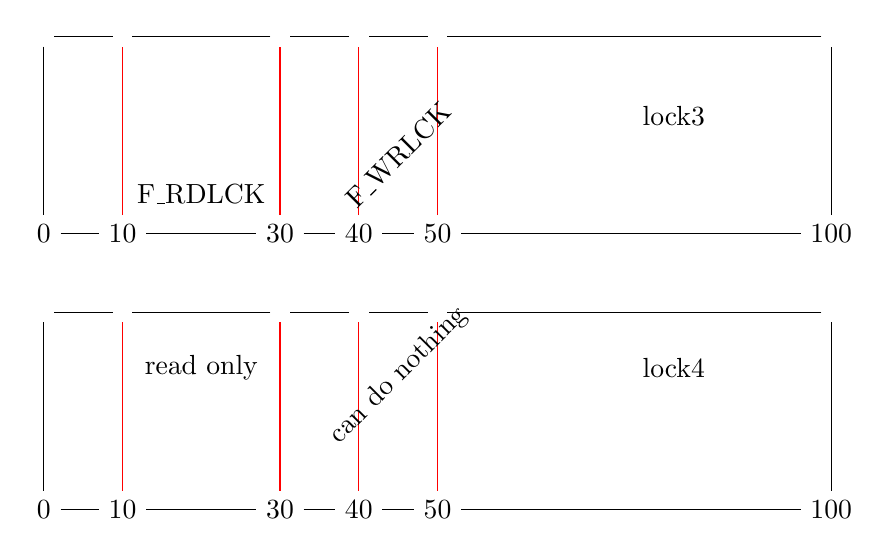
\begin{tikzpicture}
\node (a) at (0,3.5) {0} ;
\node (b) at (1,3.5) {10};
\node (c) at (3,3.5) {30};
\node (d) at (4,3.5) {40};
\node (e) at (5,3.5) {50};
\node (f) at (10,3.5) {100};
\node (g) at (10,6) {};
\node (h) at (5,6) {};
\node (i) at (4,6) {};
\node (j) at (3,6) {};
\node (k) at (1,6) {};
\node (l) at (0,6) {};
\draw (a) -- (b) --(c) -- (d) --(e) -- (f) --(g) -- (h) --(i) -- (j) --(k) -- (l) --(a);
\draw [red] (b) -- (k);
\draw [red] (c) -- (j);
\draw [red] (d) -- (i);
\draw [red] (e) -- (h);
\node (rdlck) at (2,4){F\_RDLCK}; 
\node (wrlck) at (4.5,4.5) [rotate=45]{F\_WRLCK};
\node (lock3) at (8,5){lock3}; 

\node (aa) at (0,0) {0} ;
\node (bb) at (1,0) {10};
\node (cc) at (3,0) {30};
\node (dd) at (4,0) {40};
\node (ee) at (5,0) {50};
\node (ff) at (10,0) {100};
\node (gg) at (10,2.5) {};
\node (hh) at (5,2.5) {};
\node (ii) at (4,2.5) {};
\node (jj) at (3,2.5) {};
\node (kk) at (1,2.5) {};
\node (ll) at (0,2.5) {};
\draw (aa) -- (bb) --(cc) -- (dd) --(ee) -- (ff) --(gg) -- (hh) --(ii) -- (jj) --(kk) -- (ll) --(aa);
\draw [red] (bb) -- (kk);
\draw [red] (cc) -- (jj);
\draw [red] (dd) -- (ii);
\draw [red] (ee) -- (hh);
\node (rdonly) at (2,1.8){read only}; 
\node (wrlck) at (4.5,1.7) [rotate=45]{can do nothing};
%\node (rdlck) at (2,2){F\_RDLCK}; 
%\node (wrlck) at (4.5,2) [rotate=45]{F\_WRLCK};
\node (lock4) at (8,1.8){lock4}; 
\end{tikzpicture}
\end{frame}

%------------------------------------------------
\section{数据库}
\begin{frame}
\Huge{\centerline{数据库}}
\end{frame}
%------------------------------------------------
%------------------------------------------------

\begin{frame}
\Huge{\centerline{The End}}
\end{frame}



\section{Appendix}
\begin{frame}
\Huge{\centerline{Appendix}}
\end{frame}
%----------------------------------------------------------------------------------------
\begin{frame}[fragile]
\frametitle{errno}
\label{ferr}
关于文件操作相关的错误代码所代表的错误信息可以查看:
\begin{block}{}
\begin{lstlisting}
/usr/include/sys/errno.h

\#define EEXIST          17              /* File exists */
\end{lstlisting}
\end{block}
\end{frame}
\begin{frame}{本课程相关资源下载}
\begin{enumerate}
\item
ppt

\url{https://github.com/gmsft/ppt/tree/master/linux}
\item
实验指导书

\url{https://github.com/gmsft/ppt/tree/master/book/linux}
\end{enumerate}
\end{frame}
\begin{frame}
\frametitle{about man page}
The manual is generally split into eight numbered sections, organized as follows (on Research Unix, BSD, macOS and Linux):
\begin{table}
\begin{tabular}{ll}
\toprule
\textbf{section} & \textbf{description} \\
\midrule
1 & General commands\\
 2 & System calls\\
 3& Library function(C standard library)\\
 4 & Special files(devices) and drivers\\
  5 & File formats and conventions\\
  6  & Games and screensavers\\
   7  & Miscellanea\\
   8   & System administration commands and daemons\\  
\bottomrule
\end{tabular}
\caption{man page}
\end{table}

在终端中运行man read 与 man 2 read ,观察其输出的区别。
\end{frame}

\end{document} 
